\documentclass[convert={density=300,size=1080x800,outext=.png}]{standalone}
\usepackage{tikz}
\usepackage{tikz-network}
\begin{document}
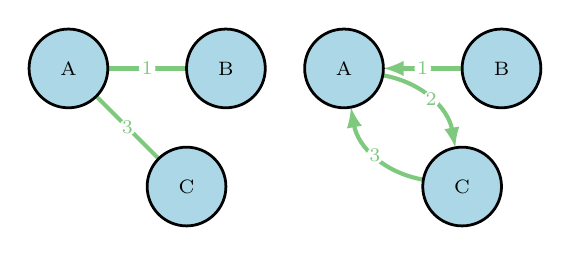
\begin{tikzpicture} 

  \Vertex[label=A, size = 1]{A} 
  \Vertex[x=2,label=B,size = 1]{B} 
  \Vertex[x=1.5,y=-1.5,label=C,size = 1]{C} 
  
  \Edge[RGB,color={127,201,127}, label=1](A)(B) 
  \Edge[RGB,color={127,201,127}, label=3](A)(C) 
  

  \Vertex[x = 3.5, label=A, size = 1]{D} 
  \Vertex[x=5.5,label=B,size = 1]{E} 
  \Vertex[x=5,y=-1.5,label=C,size = 1]{F} 
  
  \Edge[RGB,color={127,201,127},label=1,Direct](E)(D) 
  \Edge[RGB,color={127,201,127},label=2,Direct,bend=35](D)(F) 
  \Edge[RGB,color={127,201,127},label=3,Direct,bend=35](F)(D) 
  \end{tikzpicture}	

\end{document}
